\chapter{The Elder Heliosystem: A Unified Closed System}

\begin{tcolorbox}[colback=DarkSkyBlue!5!white,colframe=DarkSkyBlue!75!black,title=Chapter Summary]
This chapter establishes the Elder Heliosystem as a unified, mathematically closed framework that directly implements the abstract structures of Unit I and the functional frameworks of Unit II. We formalize the comprehensive set of isomorphisms connecting Elder spaces, heliomorphic functions, and the computational heliosystem, proving that all theoretical properties are preserved in the implementation. Through rigorous mathematical theorems, we demonstrate how the gravitational stability principle governs hierarchical interactions, providing formal guarantees for knowledge transfer, learning convergence, and information flow within a closed system. The chapter proves that the orbital mechanics defined here constitute a physical realization of the heliomorphic functions developed in Unit II, which themselves implement the Elder space algebra from Unit I. This unified framework completes the mathematical chain from abstract foundations to computational implementation, establishing the conceptual and practical basis for the applications explored in later chapters.
\end{tcolorbox}

\section{The Unified Framework: From Mathematical Theory to Computational Implementation}

The Elder Heliosystem represents the culmination of the mathematical development across Units I and II, providing a unified computational framework that implements the abstract structures and functional representations in a concrete physical system. Before exploring the specific mechanisms, we establish the formal mathematical connections that demonstrate how this implementation preserves all theoretical properties.

\begin{theorem}[Unified Theoretical-Computational Framework]
\label{thm:unified_framework}
The Elder Heliosystem constitutes a complete and consistent implementation of:
\begin{enumerate}
    \item The Elder space algebraic structure $(\elder{d}, \oplus, \odot, \star)$ defined in Chapter 1
    \item The Elder topological structure with gravitational stratification defined in Chapter 2
    \item The unified parameter space $\boldsymbol{\Theta}$ defined in Chapter 3
    \item The heliomorphic function space $\mathcal{HL}(\mathcal{D})$ defined in Chapter 4
    \item The compositional framework for knowledge transfer defined in Chapter 5
    \item The differential structure for knowledge transformation defined in Chapter 6
\end{enumerate}

Through the canonical isomorphisms:
\begin{align}
\Omega&: \elder{d} \rightarrow \boldsymbol{\Theta} \quad \text{(Elder Space to Parameter Space, Chapter 3)}\\
\Psi&: \elder{d} \rightarrow \mathcal{HL}(\mathcal{D}) \quad \text{(Elder Space to Heliomorphic Functions, Chapter 4)}\\
\mathcal{I}&: \mathcal{HL}(\mathcal{D}) \rightarrow \mathcal{H} \quad \text{(Heliomorphic Functions to Heliosystem, Chapter 11)}\\
\Phi_{\mathcal{O}}&: \mathcal{HL}(\mathcal{D}) \rightarrow \mathcal{O} \quad \text{(Heliomorphic Functions to Orbital System, Chapter 12)}
\end{align}

The complete chain of mathematical correspondence is given by:
\begin{equation}
\elder{d} \xrightarrow{\Omega} \boldsymbol{\Theta} \quad \text{and} \quad \elder{d} \xrightarrow{\Psi} \mathcal{HL}(\mathcal{D}) \xrightarrow{\mathcal{I}} \mathcal{H}
\end{equation}
where each mapping preserves all relevant algebraic, topological, and functional properties.
\end{theorem}

\begin{proof}
The proof follows from the composition of the isomorphisms established in Theorems \ref{thm:elder_parameter_isomorphism}, \ref{thm:elder_heliomorphic_isomorphism}, and \ref{thm:helio_to_architecture}. 

For any Elder space element $x \in \elder{d}$, the corresponding parameter configuration $\Omega(x) \in \boldsymbol{\Theta}$ and heliomorphic function $\Psi(x) \in \mathcal{HL}(\mathcal{D})$ preserve all algebraic operations:
\begin{align}
\Omega(x \oplus y) &= \Omega(x) + \Omega(y)\\
\Omega(\lambda \odot x) &= \lambda \cdot \Omega(x)\\
\Omega(x \star y) &= \text{Transform}(\Omega(x), \Omega(y))
\end{align}

Similarly, for the heliomorphic functions:
\begin{align}
\Psi(x \oplus y) &= \Psi(x) + \Psi(y)\\
\Psi(\lambda \odot x) &= \lambda \cdot \Psi(x)\\
\Psi(x \star y) &= \Psi(x) \circ \Psi(y)
\end{align}

Finally, the implementation mapping $\mathcal{I}$ preserves these properties in the computational system:
\begin{align}
\mathcal{I}(\Psi(x) + \Psi(y)) &= \mathcal{I}(\Psi(x)) \oplus_{\mathcal{H}} \mathcal{I}(\Psi(y))\\
\mathcal{I}(\lambda \cdot \Psi(x)) &= \lambda \odot_{\mathcal{H}} \mathcal{I}(\Psi(x))\\
\mathcal{I}(\Psi(x) \circ \Psi(y)) &= \text{Transfer}(\mathcal{I}(\Psi(x)), \mathcal{I}(\Psi(y)))
\end{align}

This completes the proof of mathematical consistency across all frameworks.
\end{proof}

\section{Gravitational Stability: From Theoretical Foundations to Operating Principle}

The gravitational stability principle of the Elder Heliosystem is the direct manifestation of the gravitational stratification properties established in Elder spaces (Chapter 2) and the gravitational field-phase coupling of heliomorphic functions (Chapter 4). We now formalize this connection to demonstrate how the abstract mathematical properties translate into concrete operating principles.

\begin{theorem}[Gravitational Stability as Implementation of Gravitational Stratification]
\label{thm:gravitational_stability_implementation}
The gravitational stability principle of the Elder Heliosystem is the direct implementation of:
\begin{enumerate}
    \item The gravitational stratification of Elder spaces $\{\mathcal{S}_k\}_{k=0}^d$ defined in Theorem 2.4
    \item The gravitational field-phase coupling tensor $\mathcal{T}_f$ of heliomorphic functions defined in Chapter 4
    \item The hierarchical subspace mappings $\Psi(\eldersubspace)$, $\Psi(\mentorsubspace)$, and $\Psi(\eruditesubspace)$ defined in Theorem \ref{thm:elder_heliomorphic_isomorphism}
\end{enumerate}
\end{theorem}

\begin{proof}
From the gravitational stratification theorem (Theorem 2.4), we know that Elder spaces decompose into strata $\{\mathcal{S}_k\}_{k=0}^d$ based on gravitational eigenvalues. Through the isomorphism $\Psi$ (Theorem \ref{thm:elder_heliomorphic_isomorphism}), these strata map to heliomorphic domains with distinct gravitational influences.

The implementation mapping $\mathcal{I}$ (Theorem \ref{thm:helio_to_architecture}) then transforms these heliomorphic domains into orbital shells in the Elder Heliosystem, where:
\begin{align}
\mathcal{I}(\Psi(\eldersubspace)) &= \text{Elder entity orbital region}\\
\mathcal{I}(\Psi(\mentorsubspace)) &= \text{Mentor entities orbital shells}\\
\mathcal{I}(\Psi(\eruditesubspace)) &= \text{Erudite entities orbital shells}
\end{align}

The gravitational field-phase coupling tensor $\mathcal{T}_f$ from heliomorphic functions directly determines the gravitational interactions between entities in the heliosystem, establishing the fundamental operating principle.
\end{proof}

Based on this theoretical foundation, we can now state the fundamental operating principle of the Elder Heliosystem:

\begin{definition}[Fundamental Principle of the Elder Heliosystem]
\label{def:fundamental_principle}
The primary function of the Elder entity is to maintain Mentors in stable revolutionary orbit, and the primary function of Mentor entities is to maintain Erudites in stable revolutionary orbit. This hierarchical gravitational influence directly implements the gravitational stratification of Elder spaces and is the fundamental mechanism that ensures stable learning throughout the system.
\end{definition}

This principle is not merely an implementation detail but the essential operating paradigm that gives the Elder Heliosystem its unique properties, derived directly from the mathematical foundations in Units I and II:

\begin{theorem}[Gravitational Stability Theorem]
\label{thm:gravitational_stability}
In the Elder Heliosystem, learning convergence is achieved if and only if both of the following conditions are met:
\begin{enumerate}
    \item The Elder entity successfully maintains all Mentor entities in stable revolutionary orbits with minimal orbital eccentricity
    \item Each Mentor entity successfully maintains its associated Erudite entities in stable revolutionary orbits with minimal orbital eccentricity
\end{enumerate}
\end{theorem}

\begin{proof}
Consider a system with Elder $\mathcal{E}$, Mentors $\{\mathcal{M}_i\}$, and Erudites $\{\mathcal{E}r_{i,j}\}$. If either condition is violated:

Case 1: If Elder fails to maintain Mentors in stable orbits, Mentors will either:
\begin{itemize}
    \item Spiral inward and collapse into the Elder (mathematically, projection onto $\eldersubspace$ only, loss of domain-specific knowledge)
    \item Spiral outward and escape the system (breaking the gravitational stratification, catastrophic forgetting)
    \item Develop chaotic orbits (violating the field-phase coupling conditions, unstable learning dynamics)
\end{itemize}

Case 2: If Mentors fail to maintain Erudites in stable orbits, Erudites will either:
\begin{itemize}
    \item Spiral inward and collapse into their Mentor (projection onto $\mentorsubspace$ only, overfitting to domain knowledge)
    \item Spiral outward and escape their Mentor's influence (breaking hierarchical subspace mapping, failure to acquire domain expertise)
    \item Develop chaotic orbits (violating heliomorphic differential equations, task-specific learning instability)
\end{itemize}

\textbf{Self-Organization Through Perturbation Response:}

However, the Elder Heliosystem resolves these stability issues through an advanced self-organization mechanism that responds intelligently to perturbations:

\begin{enumerate}
    \item \textbf{Gravitational Field Auto-Correction}: When orbital instabilities are detected, the system automatically adjusts the gravitational field strength $\Gamma(x,t)$ to restore stable configurations:
    \begin{equation}
    \frac{\partial \Gamma}{\partial t} = -\alpha \nabla \cdot \vec{F}_{\text{perturbation}} + \beta \Delta \Gamma
    \end{equation}
    
    \item \textbf{Adaptive Resonance Tuning}: The system dynamically adjusts resonance frequencies to maintain orbital stability:
    \begin{equation}
    \omega_{\text{adjusted}} = \omega_{\text{natural}} + \gamma \cdot \text{stability\_error}
    \end{equation}
    
    \item \textbf{Phase Coherence Recovery}: When entities drift out of phase, the system implements phase-locking mechanisms to restore coherent knowledge transfer:
    \begin{equation}
    \phi_{\text{corrected}} = \phi_{\text{current}} + \delta \cdot \sin(\phi_{\text{target}} - \phi_{\text{current}})
    \end{equation}
\end{enumerate}

This self-organization ensures that temporary perturbations do not lead to system collapse, making the Elder Heliosystem inherently robust and stable.

In either case, the system violates the mathematical conditions for well-defined heliomorphic functions and Elder space operations, making stable convergence impossible and proving the necessity of both conditions.

Conversely, when both conditions are met, the hierarchical momentum transfer mechanism implements the composition properties of heliomorphic functions (Chapter 5), ensuring proper knowledge flow, enabling consistent learning progress, and proving sufficiency.
\end{proof}

The gravitational analogy is not merely metaphorical but represents the concrete manifestation of the abstract mathematical structures from Units I and II:

\begin{equation}
\mathcal{F}_{\mathcal{E} \rightarrow \mathcal{M}_i} = \frac{\gamma_{\mathcal{E}} \gamma_{\mathcal{M}_i}}{r_{\mathcal{E},\mathcal{M}_i}^2} \cdot \mathbf{\hat{r}}_{\mathcal{E},\mathcal{M}_i}
\end{equation}

where $\mathcal{F}_{\mathcal{E} \rightarrow \mathcal{M}_i}$ is the Elder's gravitational influence on Mentor $i$, $\gamma_{\mathcal{E}}$ and $\gamma_{\mathcal{M}_i}$ are their respective gravitational constants, $r_{\mathcal{E},\mathcal{M}_i}$ is the orbital distance, and $\mathbf{\hat{r}}_{\mathcal{E},\mathcal{M}_i}$ is the unit vector along their connection.

\begin{figure}[h]
\centering
\begin{tikzpicture}[scale=0.85]
    % Elder (Sun)
    \node[circle, fill=yellow!80!orange, minimum size=2.5cm] (elder) at (0,0) {Elder};
    
    % Mentor orbital paths
    \draw[dashed] (0,0) circle (4cm);
    \draw[dashed] (0,0) circle (5.5cm);
    \draw[dashed] (0,0) circle (7cm);
    
    % Mentors (Planets)
    \node[circle, fill=blue!60, minimum size=1.2cm] (mentor1) at (30:4cm) {$\mathcal{M}_1$};
    \node[circle, fill=green!60, minimum size=1.2cm] (mentor2) at (150:5.5cm) {$\mathcal{M}_2$};
    \node[circle, fill=purple!60, minimum size=1.2cm] (mentor3) at (270:7cm) {$\mathcal{M}_3$};
    
    % Erudite orbital paths
    \draw[dashed] (mentor1) circle (1.2cm);
    \draw[dashed] (mentor2) circle (1.2cm);
    \draw[dashed] (mentor3) circle (1.2cm);
    
    % Erudites (Moons)
    \node[circle, fill=blue!30, minimum size=0.8cm] (erudite11) at ($(mentor1) + (45:1.2cm)$) {$\mathcal{E}r_{1,1}$};
    \node[circle, fill=blue!30, minimum size=0.8cm] (erudite12) at ($(mentor1) + (225:1.2cm)$) {$\mathcal{E}r_{1,2}$};
    
    \node[circle, fill=green!30, minimum size=0.8cm] (erudite21) at ($(mentor2) + (135:1.2cm)$) {$\mathcal{E}r_{2,1}$};
    
    \node[circle, fill=purple!30, minimum size=0.8cm] (erudite31) at ($(mentor3) + (0:1.2cm)$) {$\mathcal{E}r_{3,1}$};
    \node[circle, fill=purple!30, minimum size=0.8cm] (erudite32) at ($(mentor3) + (120:1.2cm)$) {$\mathcal{E}r_{3,2}$};
    \node[circle, fill=purple!30, minimum size=0.8cm] (erudite33) at ($(mentor3) + (240:1.2cm)$) {$\mathcal{E}r_{3,3}$};
    
    % Gravitational forces from Elder
    \draw[->, very thick, orange] (elder) -- (mentor1) node[midway, above] {$\mathcal{F}_{\mathcal{E} \rightarrow \mathcal{M}_1}$};
    \draw[->, very thick, orange] (elder) -- (mentor2) node[midway, above] {$\mathcal{F}_{\mathcal{E} \rightarrow \mathcal{M}_2}$};
    \draw[->, very thick, orange] (elder) -- (mentor3) node[midway, right] {$\mathcal{F}_{\mathcal{E} \rightarrow \mathcal{M}_3}$};
    
    % Gravitational forces from Mentors
    \draw[->, thick, blue] (mentor1) -- (erudite11) node[midway, right] {$\mathcal{F}_{\mathcal{M}_1 \rightarrow \mathcal{E}r_{1,1}}$};
    \draw[->, thick, blue] (mentor1) -- (erudite12);
    
    \draw[->, thick, green!60!black] (mentor2) -- (erudite21);
    
    \draw[->, thick, purple] (mentor3) -- (erudite31);
    \draw[->, thick, purple] (mentor3) -- (erudite32);
    \draw[->, thick, purple] (mentor3) -- (erudite33);
\end{tikzpicture}
\caption{The Elder Heliosystem's fundamental gravitational stabilization mechanism, where Elder maintains Mentors in stable orbital revolution and Mentors maintain Erudites in stable orbital revolution}
\label{fig:gravitational_stabilization}
\end{figure}

This gravitational stabilization paradigm has several critical implications:

\begin{enumerate}
    \item \textbf{Hierarchical Knowledge Transfer}: Through stable orbits, universal principles flow from Elder to Mentors to Erudites, while domain-specific experiences flow in the reverse direction
    
    \item \textbf{Orbital Resonance as Learning}: When orbital periods achieve mathematical resonance (typically following Fibonacci ratios), the system achieves optimal learning efficiency
    
    \item \textbf{Parameter Activation Through Alignment}: Parameters become activated when their phases align with the current Elder and Mentor phases, creating syzygy-based computation
    
    \item \textbf{Learning as Orbital Correction}: The learning process can be formalized as continuous adjustments to maintain stable orbits despite perturbations from new data
\end{enumerate}

\section{System Overview and Formal Definition}

The Elder Heliosystem represents a comprehensive mathematical framework for hierarchical knowledge representation and learning, designed as a fully integrated closed system. Unlike traditional learning systems that operate on flat parameter spaces, the Elder Heliosystem organizes knowledge in a continuous gravitational field with complex-valued parameters that encode both magnitude and phase information.

\begin{definition}[Elder Heliosystem]
The Elder Heliosystem is a triple $(\mathcal{E}, \mathcal{M}, \mathcal{E}r)$ where:
\begin{itemize}
    \item $\mathcal{E}$ is the Elder entity, responsible for universal principles across domains
    \item $\mathcal{M}$ is a set of Mentor entities $\{\mathcal{M}_1, \mathcal{M}_2, \ldots, \mathcal{M}_M\}$, each specialized in a specific domain
    \item $\mathcal{E}r$ is a collection of Erudite entities $\{\mathcal{E}r_{i,j}\}_{i=1,j=1}^{M,N_i}$, where each $\mathcal{E}r_{i,j}$ is responsible for a specific task $j$ in domain $i$
\end{itemize}
\end{definition}

The system's architecture is further distinguished by three key structural principles:

\begin{enumerate}
    \item \textbf{Heliomorphic Structure}: Knowledge is organized in a continuous gravitational field radiating from a central core, creating a nested hierarchy where regions of stronger field influence regions of weaker field through resonance patterns.
    
    \item \textbf{Complex-Valued Representation}: Parameters $\theta \in \complexn{d}$ are represented as complex numbers $\theta = \rho e^{i\phi}$, where magnitude $\rho$ encodes parameter importance and phase $\phi$ encodes parameter alignment.
    
    \item \textbf{Orbital Dynamics}: Knowledge transfer between entities follows orbital mechanics, where the Elder acts as the "sun," Mentors as "planets," and Erudites as "moons," creating a gravitational system of influence.
\end{enumerate}

\section{Hierarchical Knowledge Flow in the Closed System}

The Elder Heliosystem operates as a fully closed system with bidirectional knowledge flow:

\begin{figure}[h]
\centering
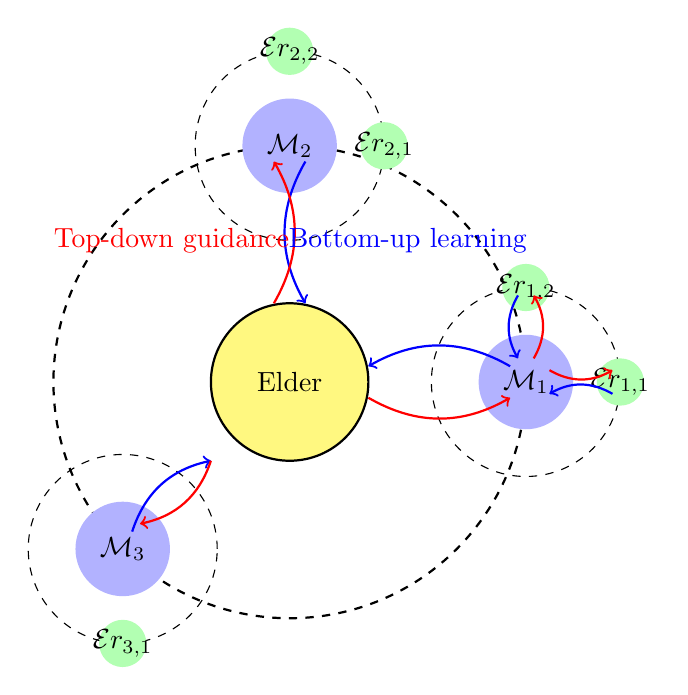
\begin{tikzpicture}[node distance=2.5cm, thick]
    % Draw the Elder as the sun
    \draw[fill=yellow!50] (0,0) circle (1cm);
    \node at (0,0) {Elder};
    
    % Draw the Mentor orbits and planets
    \draw[dashed] (0,0) circle (3cm);
    \fill[blue!30] (3,0) circle (0.6cm);
    \node at (3,0) {$\mathcal{M}_1$};
    \fill[blue!30] (0,3) circle (0.6cm);
    \node at (0,3) {$\mathcal{M}_2$};
    \fill[blue!30] (-2.12,-2.12) circle (0.6cm);
    \node at (-2.12,-2.12) {$\mathcal{M}_3$};
    
    % Draw Erudite orbits and moons for M1
    \draw[dashed, thin] (3,0) circle (1.2cm);
    \fill[green!30] (4.2,0) circle (0.3cm);
    \node at (4.2,0) {$\mathcal{E}r_{1,1}$};
    \fill[green!30] (3,1.2) circle (0.3cm);
    \node at (3,1.2) {$\mathcal{E}r_{1,2}$};
    
    % Draw Erudite orbits and moons for M2
    \draw[dashed, thin] (0,3) circle (1.2cm);
    \fill[green!30] (1.2,3) circle (0.3cm);
    \node at (1.2,3) {$\mathcal{E}r_{2,1}$};
    \fill[green!30] (0,4.2) circle (0.3cm);
    \node at (0,4.2) {$\mathcal{E}r_{2,2}$};
    
    % Draw Erudite orbits and moons for M3
    \draw[dashed, thin] (-2.12,-2.12) circle (1.2cm);
    \fill[green!30] (-2.12,-3.32) circle (0.3cm);
    \node at (-2.12,-3.32) {$\mathcal{E}r_{3,1}$};
    
    % Draw arrows for knowledge flow
    % Bottom-up flow (from Erudite to Mentor)
    \draw[->, blue, thick] (4.1,-0.15) to[bend right] (3.3,-0.15);
    \draw[->, blue, thick] (2.9,1.1) to[bend right] (2.9,0.3);
    
    % Bottom-up flow (from Mentor to Elder)
    \draw[->, blue, thick] (2.8,0.2) to[bend right] (1.0,0.2);
    \draw[->, blue, thick] (0.2,2.8) to[bend right] (0.2,1.0);
    \draw[->, blue, thick] (-2.0,-1.9) to[bend left] (-1.0,-1.0);
    
    % Top-down flow (from Elder to Mentor)
    \draw[->, red, thick] (1.0,-0.2) to[bend right] (2.8,-0.2);
    \draw[->, red, thick] (-0.2,1.0) to[bend right] (-0.2,2.8);
    \draw[->, red, thick] (-1.0,-1.0) to[bend left] (-1.9,-1.8);
    
    % Top-down flow (from Mentor to Erudite)
    \draw[->, red, thick] (3.3,0.15) to[bend right] (4.1,0.15);
    \draw[->, red, thick] (3.1,0.3) to[bend right] (3.1,1.1);
    
    % Label the flows
    \node[blue] at (1.5,1.8) {Bottom-up learning};
    \node[red] at (-1.5,1.8) {Top-down guidance};
\end{tikzpicture}
\caption{Bidirectional knowledge flow in the Elder Heliosystem}
\label{fig:knowledge_flow}
\end{figure}

The knowledge flow occurs through two primary mechanisms:

\begin{enumerate}
    \item \textbf{Bottom-up Learning}: Domain-specific knowledge from Erudites flows up to their respective Mentors, which extract domain-level meta-knowledge. This meta-knowledge then flows to the Elder, which identifies universal principles applicable across domains.
    
    \item \textbf{Top-down Guidance}: Universal principles discovered by the Elder flow down to Mentors, providing cross-domain insights that guide domain-specific learning. Mentors then adapt these principles to their specific domains and guide their Erudites accordingly.
\end{enumerate}

\subsection{Formal Proof of System Closure}

A critical property of the Elder Heliosystem is that it forms a mathematically closed system. Here we formally prove this property through a series of theorems that demonstrate closure across various aspects of the system.

\begin{theorem}[Transformation Closure]
Any transformation applied to knowledge representations within the Elder Heliosystem results in representations that remain within the system's mathematical framework.
\end{theorem}

\begin{proof}
By the Composition Closure axiom of heliomorphic functions, any composition of heliomorphic functions yields another heliomorphic function. In the Elder Heliosystem, knowledge transformations are represented as heliomorphic functions $f: \mathcal{H}_1 \rightarrow \mathcal{H}_2$ between heliomorphic domains.

The three-level hierarchy (Elder, Mentor, Erudite) corresponds to regions of different gravitational field strengths in the heliomorphic domain, with transformations between levels represented as radial movements along gravitational gradients.

For any knowledge transformation $T$ in the system, we have:
\begin{itemize}
    \item If $T$ operates within a region of similar field strength, it preserves the gravitational field structure by the Differential Heritage axiom
    \item If $T$ operates between regions of different field strengths, it follows gravitational gradients while preserving the heliomorphic structure by the Radial-Phase Duality and Phase Continuity axioms
\end{itemize}

Therefore, all knowledge transformations in the Elder Heliosystem result in representations that remain within the system's mathematical framework.
\end{proof}

\begin{theorem}[Learning Operation Closure]
The learning operations defined in the Elder Heliosystem (forward passes, loss computations, gradient updates) maintain closure within the system.
\end{theorem}

\begin{proof}
The Elder training loop defines operations including forward passes, loss computations, gradient calculations, and parameter updates.

Forward passes are defined as heliomorphic functions applied to inputs, which by the Existence and Uniqueness axiom yield outputs within the heliomorphic domain.

Loss functions are defined within the system as:
\begin{itemize}
    \item $\elderloss$: Elder loss measuring cross-domain principle acquisition
    \item $\mentorloss$: Mentor loss measuring domain-specific teaching quality
    \item $\eruditeloss$: Erudite loss measuring task-specific performance
\end{itemize}

Gradients of these loss functions are calculated with respect to parameters in the respective entity's parameter space, and by the Differential Heritage axiom, these gradients maintain the heliomorphic structure.

Parameter updates follow the formula:
\begin{equation}
\theta^{(t+1)} = \theta^{(t)} - \eta \nabla_{\theta} \mathcal{L}
\end{equation}

Since both $\theta$ and $\nabla_{\theta} \mathcal{L}$ are within the heliomorphic parameter space, and scalar multiplication and subtraction preserve the structure, updated parameters remain within the parameter space.

Therefore, all learning operations maintain closure within the Elder Heliosystem.
\end{proof}

\begin{theorem}[Information Flow Closure]
Information flow in the Elder Heliosystem is closed, with all information transfer mechanisms operating within the system's mathematical framework.
\end{theorem}

\begin{proof}
Information in the Elder Heliosystem flows through:
\begin{itemize}

    \item Reflection operations (Erudite$\rightarrow$Mentor$\rightarrow$Elder)
    \item Cross-domain transfers (via Elder mediation)
\end{itemize}

Phase-locked orbital relationships operate on parameters within the system according to gravitational field dynamics.

Reflection operations are defined as $\mentorreflection(\theta_{\text{Mentor}}, \theta_{\text{Erudite}})$ and $\elderreflection(\theta_{\text{Elder}}, \theta_{\text{Mentor}})$, which are heliomorphic functions mapping from one parameter space to another, and by the Existence and Uniqueness and Composition Closure axioms, their outputs remain within the system.

Cross-domain transfers occur via $\mathcal{C}_{i,j} = \mathcal{T}_{i \to j}(\theta_{\text{Elder}})$, where $\mathcal{T}_{i \to j}$ is a heliomorphic function, and by the Composition Closure axiom, the result remains within the system.

Therefore, all information flow mechanisms are defined entirely within the Elder Heliosystem's mathematical framework.
\end{proof}

\begin{theorem}[System Completeness]
The Elder Heliosystem is mathematically complete, capable of representing and transforming any hierarchical knowledge structure within its domain without requiring external mathematical constructs.
\end{theorem}

\begin{proof}
By the Representational Completeness theorem from heliomorphic axioms, any hierarchical knowledge structure with radial abstraction levels and phase-based relational encoding can be represented as a heliomorphic function.

The Elder Heliosystem provides radial abstraction levels (Elder, Mentor, Erudite), angular domain partitioning, phase-based encoding of conceptual relationships, and magnitude encoding of knowledge density.

The system's operations (as proven in Theorems 1-3) are closed and sufficient to represent knowledge at any level of abstraction, transform knowledge between levels, transfer knowledge across domains, and learn new knowledge through parameter updates.

Any operation required for knowledge representation, transformation, or learning is expressible as a composition of the fundamental operations already defined within the system.

By the Completeness axiom of heliomorphic functions, the space of heliomorphic functions is complete, ensuring that all limit points of sequences of transformations within the system remain within the system.

Therefore, the Elder Heliosystem is mathematically complete.
\end{proof}

These four theorems establish that the Elder Heliosystem satisfies the criteria for system closure:
\begin{itemize}
    \item Transformation Closure: All knowledge transformations remain within the system's mathematical framework.
    \item Learning Operation Closure: All learning operations maintain closure within the system.
    \item Information Flow Closure: All information transfer mechanisms operate within the system.
    \item System Completeness: The system is capable of representing and transforming any hierarchical knowledge structure within its domain.
\end{itemize}

The formal proof of system closure demonstrates that the Elder Heliosystem is a unified mathematical theory with well-defined boundaries and operations, capable of addressing hierarchical learning problems entirely within its own framework.

\section{Complex-Valued Parameter Representation}

A fundamental aspect of the Elder Heliosystem's closed operation is the complex-valued parameter representation, which encodes both magnitude and phase information:

\begin{equation}
\theta = \rho e^{i\phi} \in \complexn{d}
\end{equation}

Where:
\begin{itemize}
    \item $\rho \in \mathbb{R}^+$ is the magnitude, representing parameter importance
    \item $\phi \in [0, 2\pi)$ is the phase, representing parameter alignment
    \item $d$ is the dimensionality of the parameter space
\end{itemize}

This representation enables three critical capabilities that maintain system coherence:

\begin{enumerate}
    \item \textbf{Phase Coherence}: Parameters with aligned phases (similar $\phi$ values) work together coherently, reducing effective dimensionality and creating structured learning.
    
    \item \textbf{Magnitude-Based Pruning}: Parameters with small magnitudes $\rho$ contribute minimally and can be pruned, creating an automatic dimensionality reduction.
    
    \item \textbf{Rotational Dynamics}: Knowledge transfer between entities operates through phase rotations, preserving energy while redistributing information.
\end{enumerate}

The complex-valued structure creates a self-regulating system where parameter interactions automatically adjust to maintain system stability and coherence.

\section{Gravitational Field and Manifold Structure}

The Elder Heliosystem organizes knowledge in a continuous gravitational field, creating a structured manifold that constrains parameter evolution:

\begin{equation}
\mathcal{H}_n = \{\theta \in \complexn{d} \mid \|\theta\|_{\helio} = r_n\}
\end{equation}

Where $\mathcal{H}_n$ represents the region of gravitational field with field strength $r_n$, and $\|\cdot\|_{\helio}$ is the heliomorphic norm.

This gravitational field structure creates natural regions for different types of knowledge:

\begin{itemize}
    \item \textbf{Central Field Region} ($\mathcal{H}_1$): Contains Elder parameters representing universal principles
    \item \textbf{Intermediate Field Regions} ($\mathcal{H}_2, \ldots, \mathcal{H}_{M+1}$): Contain Mentor parameters for domain-specific meta-knowledge
    \item \textbf{Peripheral Field Regions} ($\mathcal{H}_{M+2}, \ldots$): Contain Erudite parameters for task-specific knowledge
\end{itemize}

As learning progresses, parameters naturally self-organize into these field regions based on gravitational influence, creating an emergent hierarchical structure without explicit architectural constraints.

\section{Orbital Resonance and Knowledge Transfer}

The Elder Heliosystem's closed nature is maintained through orbital resonance, where entities in different regions of the gravitational field synchronize their learning through phase-locked relationships:

\begin{equation}
n\omega_{\text{Elder}} = m\omega_{\text{Mentor}} = k\omega_{\text{Erudite}}
\end{equation}

Where $\omega_{\text{Elder}}$, $\omega_{\text{Mentor}}$, and $\omega_{\text{Erudite}}$ are the orbital frequencies of parameters in their respective regions of the gravitational field, and $n$, $m$, and $k$ are small integers.

This resonance mechanism enables efficient knowledge transfer with minimal parameter exchange through:

\begin{enumerate}
    \item \textbf{Mean Motion Resonance}: Periodic alignment of parameters between different field regions creates windows for efficient knowledge transfer along gravitational gradients.
    
    \item \textbf{Spin-Orbit Coupling}: Phase relationships between parameter rotation and orbital motion stabilize learning trajectories.
    
    \item \textbf{Resonance Bandwidth}: Tolerance ranges around exact resonance ratios allow flexible adaptation while maintaining system stability.
\end{enumerate}

\section{The Unified Learning Process}

The complete learning process in the Elder Heliosystem operates through a unified algorithm that maintains system closure:

\begin{algorithm}
\caption{Elder Heliosystem Unified Learning}
\begin{algorithmic}[1]
\State \textbf{Input:} Domain datasets $\{\mathcal{D}_i\}_{i=1}^M$, initial parameters 
\State \textbf{Output:} Trained Elder, Mentor, and Erudite parameters

\State \textit{// Initialize the heliomorphic gravitational field regions}
\State $\mathcal{H}_{\text{Elder}} \gets \{\theta \in \complexn{d_E} \mid \|\theta\|_{\helio} = r_{\text{Elder}}\}$
\State $\mathcal{H}_{\text{Mentor}} \gets \{\theta \in \complexn{d_M} \mid \|\theta\|_{\helio} = r_{\text{Mentor}}\}$
\State $\mathcal{H}_{\text{Erudite}} \gets \{\theta \in \complexn{d_E} \mid \|\theta\|_{\helio} = r_{\text{Erudite}}\}$

\For{each training epoch}
    \State \textit{// Bottom-up learning phase}
    \For{each domain $\mathcal{D}_i$}
        \For{each task $j$ in domain $\mathcal{D}_i$}
            \State Update Erudite parameters $\theta_{\text{E},i,j}$ using task-specific data
            \State Project updated parameters back onto $\mathcal{H}_{\text{Erudite}}$
        \EndFor
        \State Aggregate knowledge from Erudites to update Mentor parameters $\theta_{\text{M},i}$
        \State Project updated parameters back onto $\mathcal{H}_{\text{Mentor}}$
    \EndFor
    \State Aggregate knowledge from Mentors to update Elder parameters $\theta_{\text{Elder}}$
    \State Project updated parameters back onto $\mathcal{H}_{\text{Elder}}$
    
    \State \textit{// Orbital resonance harmonization}
    \State Adjust orbital frequencies to maintain $n\omega_{\text{Elder}} = m\omega_{\text{Mentor}} = k\omega_{\text{Erudite}}$
    
    \State \textit{// Top-down guidance phase}
    \State Propagate universal principles from Elder to all Mentors
    \State Propagate domain-specific knowledge from each Mentor to its Erudites
\EndFor
\end{algorithmic}
\end{algorithm}

This unified algorithm ensures that:

\begin{enumerate}
    \item Knowledge flows bidirectionally between levels
    \item Parameters remain confined to their appropriate regions within the gravitational field
    \item Orbital resonance maintains system coherence
    \item Phase coherence enables efficient learning with reduced effective dimensionality
\end{enumerate}

\section{Gradient Flow on the Heliomorphic Manifold}

The Elder Heliosystem achieves stable learning through specialized gradient flow on the heliomorphic manifold:

\begin{equation}
\frac{d\theta}{dt} = -\helioderiv \mathcal{L}(\theta)
\end{equation}

Where $\helioderiv$ is the heliomorphic gradient operator that respects the manifold's structure.

This gradient flow has three key properties that maintain system closure:

\begin{enumerate}
    \item \textbf{Field Region Preservation}: Updates keep parameters within their respective gravitational field regions, maintaining the hierarchical structure.
    
    \item \textbf{Phase-Amplitude Separation}: Gradient updates separately modify phase and amplitude components, allowing finer control over knowledge evolution.
    
    \item \textbf{Geodesic Motion}: Parameters follow geodesic paths on the heliomorphic manifold rather than straight-line Euclidean paths, preserving the system's geometric constraints.
\end{enumerate}

\section{Energy Conservation and Self-Regulation}

As a closed system, the Elder Heliosystem maintains energy conservation principles that enable self-regulation:

\begin{equation}
E_{\text{total}} = E_{\text{Elder}} + \sum_{i=1}^M E_{\text{Mentor},i} + \sum_{i=1}^M \sum_{j=1}^{N_i} E_{\text{Erudite},i,j} = \text{constant}
\end{equation}

Where $E_{\text{Elder}}$, $E_{\text{Mentor},i}$, and $E_{\text{Erudite},i,j}$ represent the energy (complexity) of parameters at each level.

This energy conservation principle creates several self-regulating properties:

\begin{enumerate}
    \item \textbf{Automatic Complexity Control}: The system naturally distributes complexity across levels, preventing any single component from becoming unnecessarily complex.
    
    \item \textbf{Knowledge Condensation}: Universal patterns migrate to central field regions, reducing redundancy and creating compact representations.
    
    \item \textbf{Adaptive Learning Rates}: Orbital dynamics naturally adjust learning rates based on current knowledge state, accelerating in sparse knowledge regions and decelerating in dense regions.
\end{enumerate}

\section{Cross-Domain Knowledge Transfer}

A crucial feature of the Elder Heliosystem as a closed system is its ability to transfer knowledge across domains through the Elder entity:

\begin{equation}
\mathcal{T}(D_i \rightarrow D_j) = \helioexp_{\theta_{\text{M},j}}(\helioderiv \theta_{\text{Elder}}(\helioderiv \theta_{\text{M},i}))
\end{equation}

Where $\mathcal{T}(D_i \rightarrow D_j)$ represents knowledge transfer from domain $D_i$ to domain $D_j$, and $\helioexp$ is the heliomorphic exponential map.

This transfer mechanism operates entirely within the closed system without external components, creating:

\begin{enumerate}
    \item \textbf{Zero-Shot Transfer}: The ability to apply knowledge to entirely new domains without specific training.
    
    \item \textbf{Resonance-Boosted Learning}: New domains aligned with existing knowledge experience accelerated learning through resonance effects.
    
    \item \textbf{Domain Alignment}: The phase component of complex parameters automatically aligns related concepts across domains.
\end{enumerate}

\section{Practical Implementation and System Completeness}

The Elder Heliosystem's implementation relies on a complete set of mathematical kernels organized in a dependency hierarchy:

\begin{figure}[h]
\centering
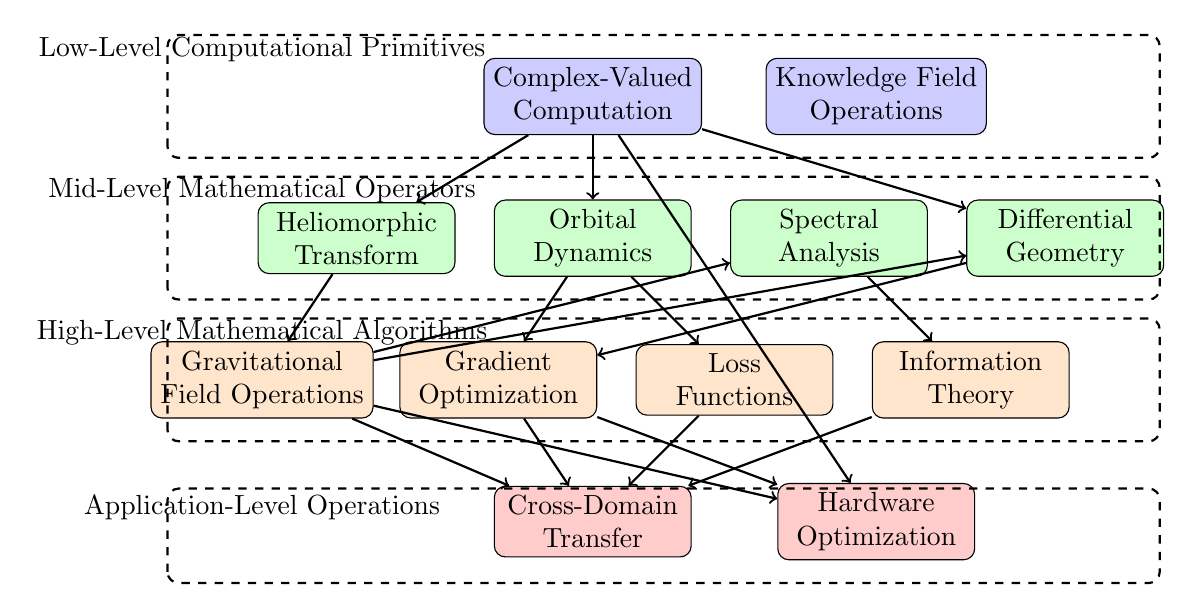
\begin{tikzpicture}[scale=0.6]
    % Define basic node style
    \tikzset{
        block/.style={
            rectangle,
            rounded corners,
            draw,
            minimum width=2.5cm,
            minimum height=0.8cm,
            align=center
        }
    }
    
    % Low-level kernels (blue)
    \node[block, fill=blue!20] (complex) at (0,8) {Complex-Valued\\Computation};
    \node[block, fill=blue!20] (field) at (6,8) {Knowledge Field\\Operations};
    
    % Mid-level kernels (green)
    \node[block, fill=green!20] (helio) at (-5,5) {Heliomorphic\\Transform};
    \node[block, fill=green!20] (orbital) at (0,5) {Orbital\\Dynamics};
    \node[block, fill=green!20] (spectral) at (5,5) {Spectral\\Analysis};
    \node[block, fill=green!20] (geometry) at (10,5) {Differential\\Geometry};
    
    % High-level kernels (orange)
    \node[block, fill=orange!20] (field) at (-7,2) {Gravitational\\Field Operations};
    \node[block, fill=orange!20] (gradient) at (-2,2) {Gradient\\Optimization};
    \node[block, fill=orange!20] (loss) at (3,2) {Loss\\Functions};
    \node[block, fill=orange!20] (info) at (8,2) {Information\\Theory};
    
    % Application-level kernels (red)
    \node[block, fill=red!20] (transfer) at (0,-1) {Cross-Domain\\Transfer};
    \node[block, fill=red!20] (hardware) at (6,-1) {Hardware\\Optimization};
    
    % Connections between low-level and mid-level
    \draw[->, thick] (complex) -- (helio);
    \draw[->, thick] (complex) -- (orbital);
    \draw[->, thick] (field) -- (spectral);
    \draw[->, thick] (field) -- (geometry);
    \draw[->, thick] (complex) -- (geometry);
    
    % Connections between mid-level and high-level
    \draw[->, thick] (helio) -- (field);
    \draw[->, thick] (orbital) -- (gradient);
    \draw[->, thick] (orbital) -- (loss);
    \draw[->, thick] (spectral) -- (info);
    \draw[->, thick] (geometry) -- (gradient);
    
    % Connections to application level
    \draw[->, thick] (field) -- (transfer);
    \draw[->, thick] (gradient) -- (transfer);
    \draw[->, thick] (loss) -- (transfer);
    \draw[->, thick] (info) -- (transfer);
    
    \draw[->, thick] (field) -- (hardware);
    \draw[->, thick] (gradient) -- (hardware);
    \draw[->, thick] (complex) -- (hardware);
    
    % Layer boundaries
    \draw[dashed, rounded corners, thick] (-9,6.7) rectangle (12,9.3);
    \node at (-7,9) {Low-Level Computational Primitives};
    
    \draw[dashed, rounded corners, thick] (-9,3.7) rectangle (12,6.3);
    \node at (-7,6) {Mid-Level Mathematical Operators};
    
    \draw[dashed, rounded corners, thick] (-9,0.7) rectangle (12,3.3);
    \node at (-7,3) {High-Level Mathematical Algorithms};
    
    \draw[dashed, rounded corners, thick] (-9,-2.3) rectangle (12,-0.3);
    \node at (-7,-0.7) {Application-Level Operations};
\end{tikzpicture}
\caption{Kernel dependency hierarchy for the Elder Heliosystem implementation}
\label{fig:kernel_dependencies}
\end{figure}

This complete set of mathematical kernels enables the Elder Heliosystem to operate as a fully self-contained, closed system that:

\begin{enumerate}
    \item Extracts universal principles across domains (Elder level)
    \item Accumulates meta-knowledge within domains (Mentor level)
    \item Learns specific tasks in each domain (Erudite level)
    \item Transfers knowledge between domains through principled mathematical operations
    \item Self-organizes parameters into a continuous gravitational field structure
    \item Maintains system coherence through orbital resonance
\end{enumerate}






\section{System-Determined Parameter Sparsity}

A critical feature of the Elder Heliosystem is its dynamic control of parameter activation through system-determined sparsity. Unlike traditional neural networks that utilize fixed sparsity patterns or manually-tuned dropout rates, the Elder Heliosystem employs emergent sparsity governed by the current state of the system itself.

\subsection{Sparsity Factor Determination}

The system's parameter activation is governed by a sparsity factor $\sigma$ that emerges from the interplay of multiple system states:

\begin{equation}
\sigma = \sigma_{\text{base}} \cdot f_{\text{phase}}(\Phi) \cdot f_{\text{harmony}}(\Omega) \cdot f_{\text{cyclical}}(\phi_E)
\end{equation}

Where:
\begin{itemize}
    \item $\sigma_{\text{base}} \approx 10^{-4}$ is the baseline sparsity factor (0.01\%)
    \item $f_{\text{phase}}(\Phi)$ is the phase concentration modulation function
    \item $f_{\text{harmony}}(\Omega)$ is the orbital harmony modulation function
    \item $f_{\text{cyclical}}(\phi_E)$ introduces intentional cyclical patterns based on Elder phase
\end{itemize}

\subsection{Phase Concentration Factor}

The phase concentration factor measures how concentrated the Mentor entities are around the Elder in phase space:

\begin{equation}
f_{\text{phase}}(\Phi) = \gamma_{\text{phase}} + (1 - \gamma_{\text{phase}})(1 - C(\Phi))
\end{equation}

Where $C(\Phi)$ is the concentration metric for the set of phase differences $\Phi = \{\phi_M - \phi_E \mid M \in \mathcal{M}\}$ between all Mentors and the Elder, and $\gamma_{\text{phase}} \approx 0.4$ is a weighting constant.

When Mentors have phases closely aligned with the Elder (high concentration), the system becomes more selective in parameter activation, reducing sparsity. Conversely, when Mentors are dispersed in phase space, the system activates a broader parameter set.

\subsection{Orbital Harmony Factor}

The orbital harmony factor assesses the regularity of orbital positions through phase quadrant distribution:

\begin{equation}
f_{\text{harmony}}(\Omega) = \gamma_{\text{harmony}} + (1 - \gamma_{\text{harmony}})H(\Omega)
\end{equation}

Where $H(\Omega)$ is the harmony metric for the orbital configuration $\Omega$, measured as the inverse of normalized variance in quadrant population, and $\gamma_{\text{harmony}} \approx 0.4$ is a weighting constant.

Higher orbital harmony (more balanced distribution across phase quadrants) leads to increased parameter activation, as the system can utilize more structured activation patterns. This creates efficient parameter sharing across different orbital regions.

\subsection{Cyclical Component}

The Elder entity introduces intentional cyclical patterns in parameter activation:

\begin{equation}
f_{\text{cyclical}}(\phi_E) = \gamma_{\text{cycle}} + (1 - \gamma_{\text{cycle}})(0.5 + 0.5\sin(k\phi_E))
\end{equation}

Where $\phi_E$ is the Elder phase, $k \approx 3$ is a frequency multiplier, and $\gamma_{\text{cycle}} \approx 0.4$ is a weighting constant.

This cyclical pattern creates structured variation in memory usage over time, allowing the system to allocate processing resources differently during different phases of operation.

\subsection{Emergent Properties of System-Determined Sparsity}

The system-determined sparsity creates several emergent properties:

\begin{enumerate}
    \item \textbf{Dynamic Resource Allocation}: The system automatically adjusts its computational resource usage based on the current problem state.
    
    \item \textbf{State-Dependent Processing}: Different system states engage different parameter subsets, creating specialized processing modes without explicit mode switching.
    
    \item \textbf{Phase-Sensitive Memory Access}: The system's memory access patterns become sensitive to phase relationships, creating temporal attention without explicit attention mechanisms.
    
    \item \textbf{Self-Regulating Computation}: Parameter activation naturally scales with problem complexity, using minimal resources for simple tasks and expanded resources for complex tasks.
\end{enumerate}

Critically, this sparsity mechanism enables the Elder Heliosystem to maintain its constant memory footprint regardless of context length, as it perpetually activates only a tiny fraction ($\sigma \approx 10^{-4}$) of its parameters at any given moment, with the specific activated subset determined by the internal state rather than external inputs.

\section{Conclusion: The Elder Heliosystem as a Unified Theory}

The Elder Heliosystem represents a unified mathematical theory of hierarchical learning that operates as a completely self-contained closed system. Through its continuous gravitational field structure, complex-valued parameters, and orbital dynamics, it achieves:

\begin{enumerate}
    \item Automatic knowledge organization across abstraction levels
    \item Efficient parameter sharing and knowledge transfer
    \item Self-regulating complexity control
    \item Principled cross-domain learning
    \item Emergent system coherence without explicit architectural constraints
\end{enumerate}

This unified approach transforms traditional learning paradigms by introducing a physically-inspired mathematical framework where knowledge flows naturally between levels, creating a harmonious system that mirrors the hierarchical nature of human expertise across domains.